\chapter{Un poquito (casi nada) de Astronomía}
\label{cap:poquito-de-astronomia}

\vfill

\lettrine[lines=2]{C}{ecilia y Antonia} caminaban morosamente por los
jardines de Harvard. El otoño se encontraba avanzado, pero el Sol de
la tarde alcanzaba para acariciarlas suavemente. Hojas secas, doradas
y carmesíes, danzaban capichosamente a su paso al aire impuesto por
una brisa imprevista y veleidosa. Ensimismadas en sus pensamientos,
compartían el delicado e íntimo don del silencio enriquecido y poblado
por el afecto.

Cecilia se detuvo con suavidad. Cerrando los párpados, levantó el
rostro al cielo para sentir los rayos de Sol filtrándose entre las
ramas de los árboles añosos de Harvard. La leve caricia solar le
recordó el comienzo de esta aventura; abriendo los ojos dirigió la
mirada a su amiga:

---Antonia, creo que es momento de que discutamos el valor del ángulo
que debe recibir el módulo \lstinline!digito! a fin de seguir
fiel\-men\-te la dirección del Sol en el cielo.

Antonia asintió con un gesto que tal vez era de resignación. Juntas
retomaron su paseo entre las hojas caídas y danzantes, los árboles, la
brisa y los rayos de Sol.

%\vfill

\section{El giro de la Tierra}

Antonia recorrió con su mirada el jardín a su alrededor. Parecía a
punto de lanzar una proclama al mundo entero; con voz firme, anunció:

---La Tierra gira sobre sí misma, alrededor de una línea imaginaria
que llamamos `eje del mundo'.

Cecilia abrió grandes los ojos, y llevándose una mano al pecho,
exclamó:

---¡No! ¿En serio?

Ambas amigas se permitieron reír levemente: ese tipo de bromas
sobreactuadas las divertían mucho.

---Pues sí, doctora; así es ---confirmó Antonia, inclinando
ligeramente la cabeza---. Pero, claro: la percepción inmediata que se
ofrece a nuestros sentidos es muy otra y simétrica: a nosotras,
ingenuas observadoras terrestres, nos parece que es el cielo el que
gira alrededor nuestro: estrellas, planetas y nebulosas en coordinada
y diaria danza. Y de esa coreografía incesante, por supuesto, también
participa nuestra querida estrella particular: el Sol.

\section{El giro aparente del Sol}

Cecilia evocó con nostalgia sus primeras lecciones de Astronomía. Como
en toda primera aproximación a una materia nueva, no había aprendido
mucho, naturalmente. Además, su profesor inicial había sido Luis
López, que garantizaba con sus exposiciones lentas, desorganizadas y
ambiguas la confusión y la perplejidad. A pesar de eso y
misteriosamente, su entusiasmo por la Astronomía no decayó y pudo
conquistarla luego con eficacia y profundidad.

El giro de la Tierra sobre su propio eje se refleja como una rotación
aparente del cielo en sentido contrario; aún conservaba entre sus
viejos apuntes algunos dibujos que Luis hacía pasar por
explicaciones. Previendo que en este capítulo discutirían el tema,
consideró conveniente llevar su carpeta de aquel curso al paseo por
los jardines. Encontró rápidamente la figura \ref{fig:mov-ap}: en ella
se adivinaba un observador parado sobre la Tierra ---a la que siente
inmóvil bajo sus pies--- mientras el cielo (que puede considerarse,
con un modelo simplista pero efectivo, como una esfera en cuyo centro
se encuentra) gira a su alrededor en el término de un día y de este a
oeste ---contrariamente al giro real de la Tierra de oeste a este
sobre su propio eje.

\begin{figure}[t]
  \centering
  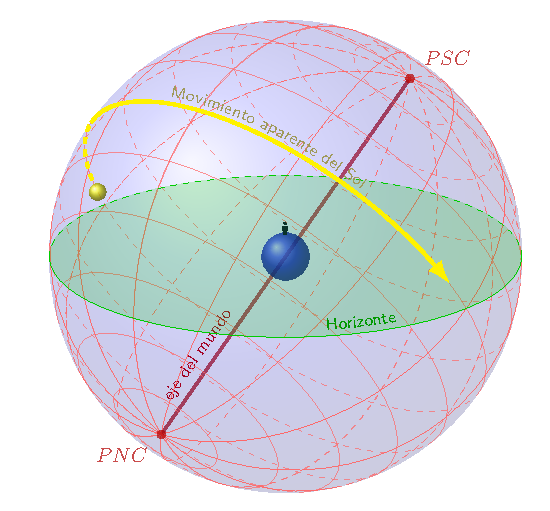
\includegraphics[width=.5\textwidth]{imagenes/movimiento-aparente-solar}
  \caption{Movimiento diurno aparente del Sol, representado sobre el
    modelo de la esfera celeste. $PSC$ y $PNC$ son los polos celestes
    sur y norte, respectivamente: proyecciones en el cielo de los
    homónimos polos terrestres, y extremos del eje alrededor del cual
    nuestro planeta gira. La Tierra y el observador, naturalmente, se
    hallan fuera de escala: en comparación con la esfera que
    representa el cielo, observador y planeta no son más que un
    ínfimo punto central, inmerso en el plano del horizonte.  }
  \label{fig:mov-ap}
\end{figure}


\section{La posición del reloj}


---Como recordarás ---dijo Antonia mirando el dibujo que Cecilia tenía
en sus manos---, el cuerpo de nuestro reloj será un semicilindro
horadado de manera tal de transformar la luz del Sol en rayos
discretos que configuren los dígitos que indicarán la hora actual
debajo del mismo.

\begin{figure}[ht]
  \centering
     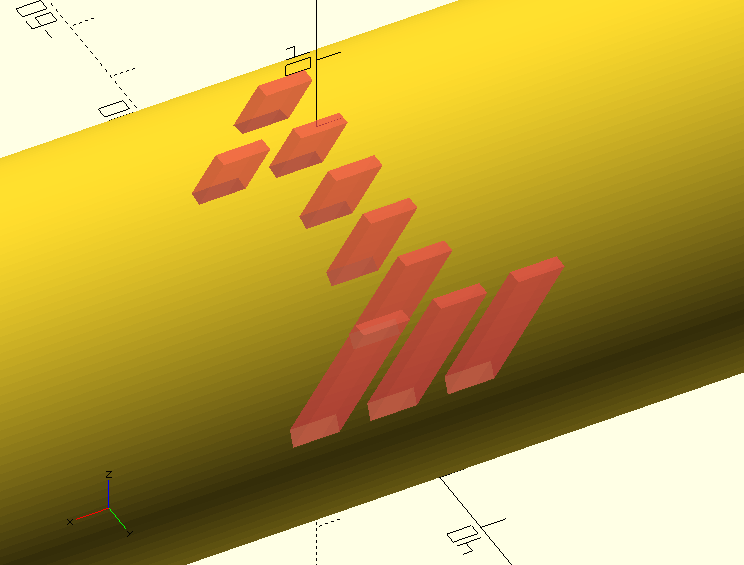
\includegraphics[width=.47\textwidth]{imagenes/digito-corte-1}\hfill
     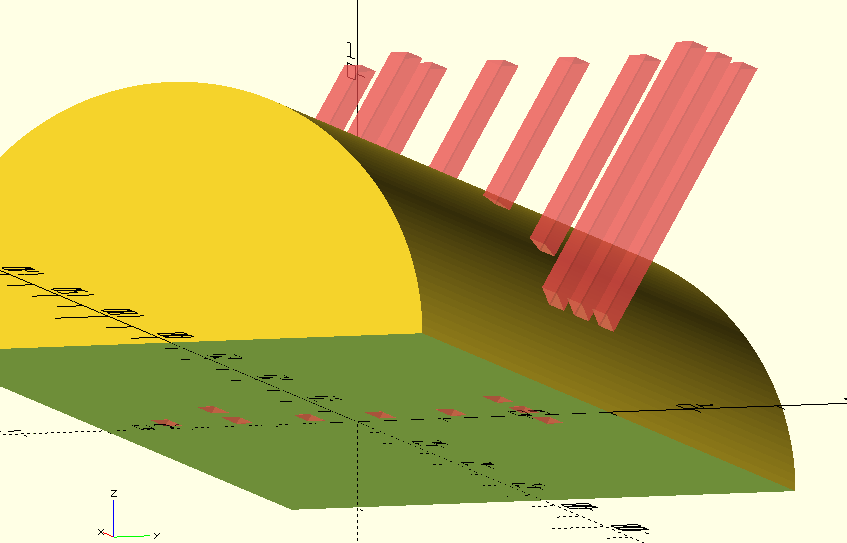
\includegraphics[width=.47\textwidth]{imagenes/digito-corte-2}
     \caption{Los orificios en el reloj deben permitir que los rayos
       de Sol indiquen la hora correcta.}
     \label{fig:orificios-correctos}
\end{figure}

Antonia se detuvo, mientras parecía buscar la mejor manera de
proseguir:

---Nosotras, entonces, queremos que el Sol, en su movimiento diario,
`gire' también alrededor de nuestro reloj.  Así, a medida que el
ángulo que forma el Sol con la base del semicilindro cambia, cambiarán
también los agujeros con que debemos perforarlo.

---En otras palabras ---concluyó Cecilia---, debemos colocar el eje
del semicilindro paralelamente al eje del mundo, puesto que el Sol
parece girar alrededor del mismo.


\begin{figure}[ht]
  \centering
  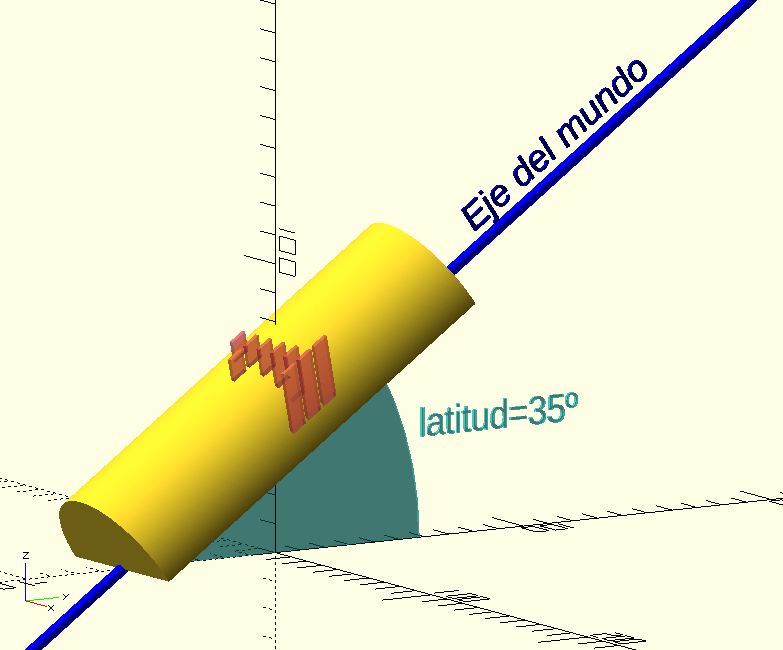
\includegraphics[width=.45\textwidth]{imagenes/inclinacion-reloj}  
  \caption[Inclinación del reloj.]{El cuerpo del reloj debe ser
    ubicado paralelamente al eje de la Tierra, puesto que queremos que
    el Sol gire, de manera aparente, alrededor del mismo.}
  \label{fig:inclinacion-reloj}
\end{figure}

Antonia aprobó, asintiendo con un movimiento de cabeza:

---El eje del mundo, como seguramente tendrás en algún lugar de tus
apuntes, forma con el horizonte un ángulo igual a la latitud del lugar
donde una se encuentra ---Antonia suspiró con hastío---. ¡A Luis le
encanta demostrarlo!

Cecilia lo confirmó alzando los ojos, con un gesto de cansancio
sobreactuado.

Antonia se dirigió con paso ligero a un banco cercano; en los suyos
flotaba ahora una expresión divertida.

---A mí me gustan dos casos particulares ---dijo, mientras se
recostaba boca arriba sobre el largo banco de ma\-de\-ra---. Si estás
ubicada en un punto cualquiera de la línea del Ecuador, el eje del
mundo yace en el horizonte, y los astros se mueven entonces
aparentemente de manera perpendicular a ese plano.


Antonia movía los brazos de manera perpendicular al piso, describiendo
círculos tan amplios como su sonrisa.


\begin{figure}[ht]
  \centering
  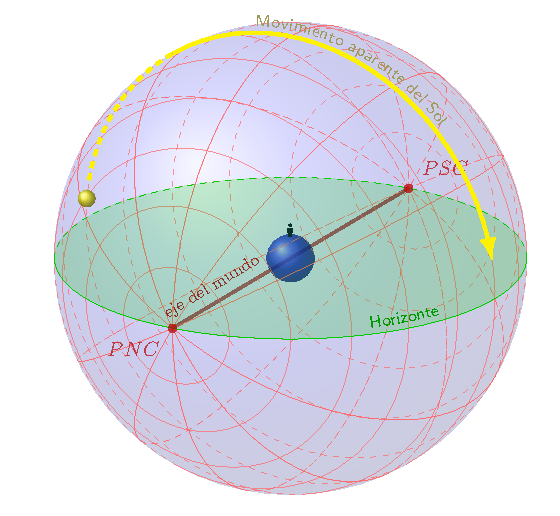
\includegraphics[width=.44\textwidth]{imagenes/movimiento-aparente-solar-ecuador}
  \caption{Movimiento diurno aparente del Sol, tal como es apreciado
    por un observador ubicado en el Ecuador terrestre.}
  \label{fig:mov-ap-ec}
\end{figure}




Cecilia, sin saber muy bien porqué, extendió también los suyos, pero
horizontalmente hacia los costados mientras, de pie junto al banco,
comenzaba a girar lentamente sobre sí misma:

---Mientras que si te hallaras en uno de los polos de la Tierra, el
eje del mundo sería perpendicular a tu horizonte y las estrellas
girarían así a tu alrededor.

\begin{figure}[ht]
  \centering
  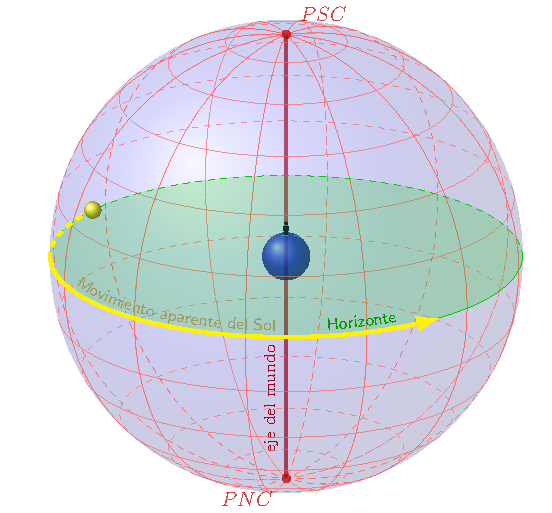
\includegraphics[width=.45\textwidth]{imagenes/movimiento-aparente-solar-polos}
  \caption{Movimiento diurno aparente del Sol, tal como es apreciado
    por un observador ubicado en el polo sur terrestre.}
  \label{fig:mov-ap-pol}
\end{figure}

Cecilia, tras varias vueltas sobre sí misma, simuló con suma gracia
que sentía un mareo; su cuerpo se bamboleó exageradamente a un lado y
otro, y se desplomó sobre el banco en el que Antonia, riendo, ya se
había incorporado.

Cuando el eco de sus risas se apagó, confundiéndose con el rumor de
las hojas que seguían bailando con la brisa y los rayos de Sol,
Cecilia juzgó apropiado afrontar la cuestión del ángulo:

---¿Y, Antonia? Ya sabemos cómo orientar nuestro reloj, pero ¿qué
hacemos con el dichoso ángulo para formar los dígitos?

En lugar de la respuesta esperada, encontró que Antonia estaba
contemplando ahora las figuras \ref{fig:mov-ap}, \ref{fig:mov-ap-ec} y
\ref{fig:mov-ap-pol} con gesto de desaprobación:

---Ahora vamos, Cecilia ---protestó---; ¡pero no me digas que Luis les
contó que el Sol se encuentra siempre equidistante de ambos polos
celestes!

---¡Por supuesto que no! ---respondió Cecilia, riendo---.  ¡El curso
no era \emph{tan} malo! Alcanzamos a ver que, debido a la inclinación
del eje terrestre, el Sol durante el año se acerca alternativamente al
polo norte y al polo sur celestes, separándose del plano del ecuador
celeste\footnote{Llámase \emph{ecuador celeste} al plano perpendicular
  al eje del mundo y equidistante de ambos polos celestes.} hasta un
máximo de unos 23,5$^{\circ}$.

Tras unos instantes, encontró la prueba:

---¿Ves? Acá tengo las figuras \ref{fig:mov-ap-pol-21-dic} y
\ref{fig:mov-ap-21-jun}: en ambas podés ver el Sol surcando el cielo
ora más cerca del polo sur celeste, ora más cerca del polo opuesto.

\begin{figure}[ht]
\begin{minipage}[t]{0.5\textwidth}
  \centering
  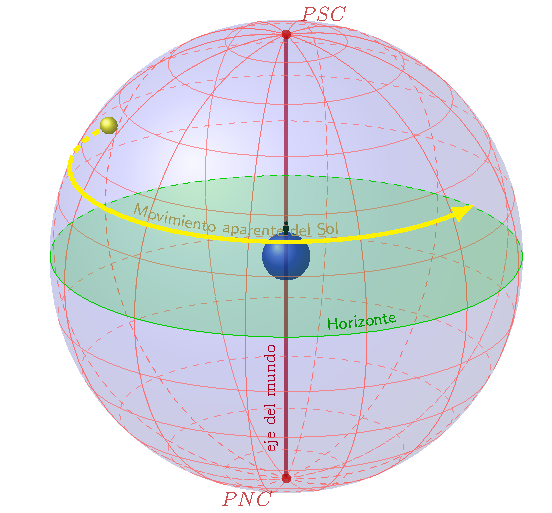
\includegraphics[width=.9\textwidth]{imagenes/movimiento-aparente-solar-polos-21-dic}
  \captionsetup{width=.9\textwidth}
  \caption{Movimiento diurno aparente del Sol, visto desde el polo sur
    terrestre el 21 de diciembre.}
  \label{fig:mov-ap-pol-21-dic}
\end{minipage}%
\begin{minipage}[t]{0.5\textwidth}
 \centering
 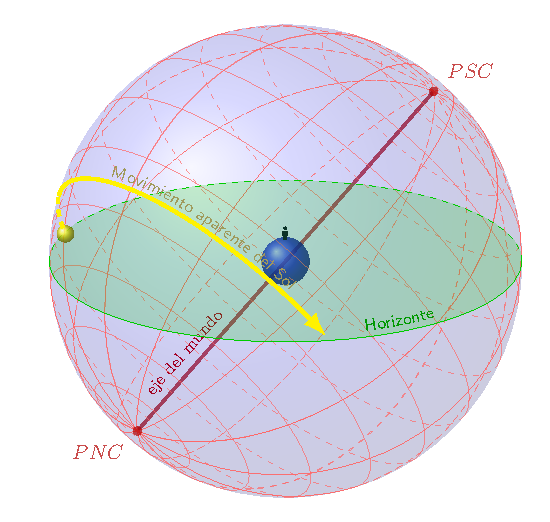
\includegraphics[width=.9\textwidth]{imagenes/movimiento-aparente-solar-21-jun}
   \captionsetup{width=.9\textwidth}
   \caption{Movimiento diurno aparente del Sol, visto desde una
     latitud de 35$^{\circ}$S el 21 de junio.}
  \label{fig:mov-ap-21-jun}
\end{minipage}
\end{figure}


---Bien ---Antonia aprobó displicentemente---. En cualquier caso, el
movimiento aparente del Sol, sin importar qué tan cerca se encuentre
de cada polo celeste, discurre diariamente en un plano perpendicular
al eje del mundo, o sea, en un \emph{paralelo celeste}; así que
nuestra conclusión anterior acerca de la orientación del reloj no
cambia: debemos colocarlo paralelamente al eje terrestre.

Cecilia pareció ofuscarse ligeramente:

---Nunca discutí eso, creo.

---No, está bien ---insitió Antonia---; sólo lo aclaraba.

---Pues no hacía falta ---replicó Cecilia, contrariada.

\section{El dichoso ángulo}


Levantándose del banco, retomaron su lento paseo en silencio. Tras
unos instantes, Antonia creyó conveniente retomar la cuestión del
ángulo:

---Podemos llamar \emph{día solar} a una rotación aparente completa
del Sol alrededor nuestro. Resulta cómodo dividirlo en 24 partes, dado
que ese número tiene muchos divisores.

---Es la misma razón por la que las medialunas se venden por docena:
la capacidad del número 12 para dividirse en partes enteras promueve
la concordia de familias y grupos de amigos ---agregó
Cecilia---. Bueno, salvo que los comensales sean cinco o diez...

---Por esa razón es tan popular el número 60: tiene los mismos
divisores que 12, pero también los de 10. Aunque creo que una
`sesentena' de medialunas excedería el presupuesto de casi cualquier
familia ---admitió Antonia---. En cualquier caso, a esas 24 partes las
llamamos \emph{horas}.

---Y de esas 24, decidimos que la hora 12 coincida con la posición más
alta que adquiere el Sol en su movimiento aparente, y la hora 0 con la
opuesta ---añadió Cecilia.

---Exacto ---aprobó Antonia---. De hecho, a esas posiciones del Sol
las llamamos \emph{culminación superior} y \emph{culminación
  inferior}, respectivamente.


\begin{figure}[ht]
  \centering
  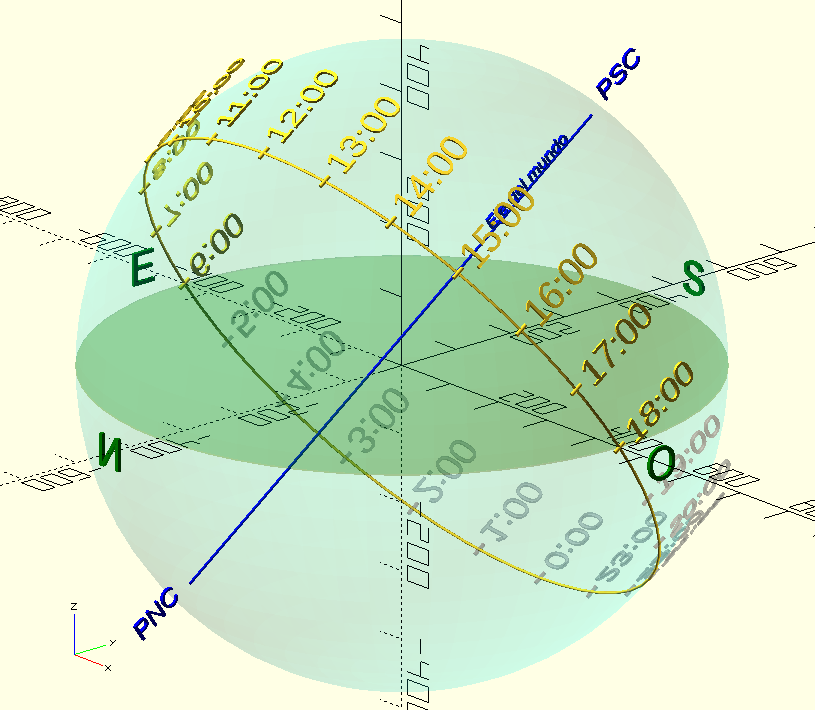
\includegraphics[width=.6\textwidth]{imagenes/esfera-celeste-horas-sur}
  \caption{El ecuador celeste divido según las horas ocupadas por el
    Sol en su movimiento aparente diurno.}
  \label{fig:horas-sur}
\end{figure}

\begin{figure}[ht]
  \centering
  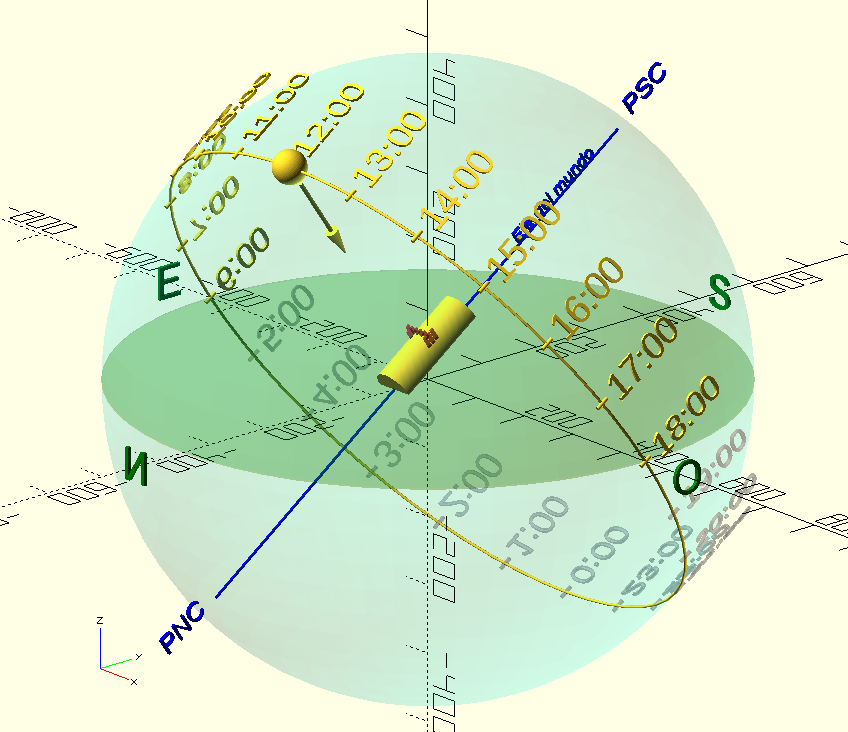
\includegraphics[width=.5\textwidth]{imagenes/sol-culminacion-superior}\hfill
   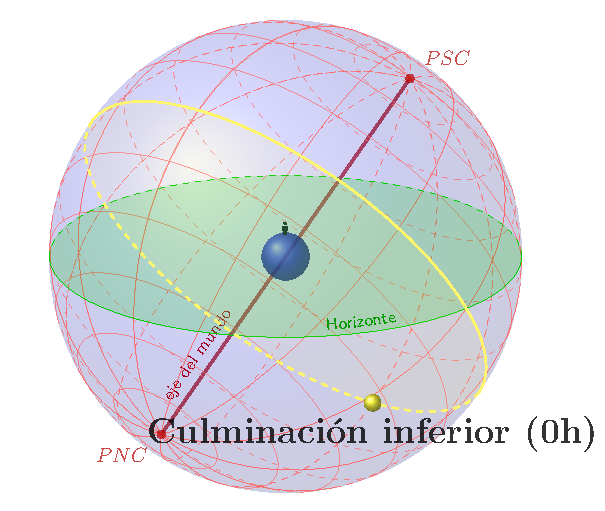
\includegraphics[width=.5\textwidth]{imagenes/sol-culminacion-inferior}  
   \caption{El Sol en sus culminaciones superior e inferior.}
  \label{fig:culminaciones}
\end{figure}


Cecilia sonrió maliciosamente:

---Claro ---dijo, procurando que su tono de voz no sonara demasiado
picante, a la vez que buscaba en su carpeta---. Mirá; acá están: en la
figura \ref{fig:culminaciones} se aprecian ambas culminaciones.


Antonia miró fijamente a Cecilia:

---Está bien ---admitió---; parece que algunas cosas vieron en ese
curso. En todo caso ---prosiguió, acelerando un poco el paso---, creo
que ya estamos en condiciones de determinar, para cada hora solar, el
ángulo que los rayos de Sol formarán con el semicilindro de nuestro
reloj.

\begin{figure}[ht]
  \centering
  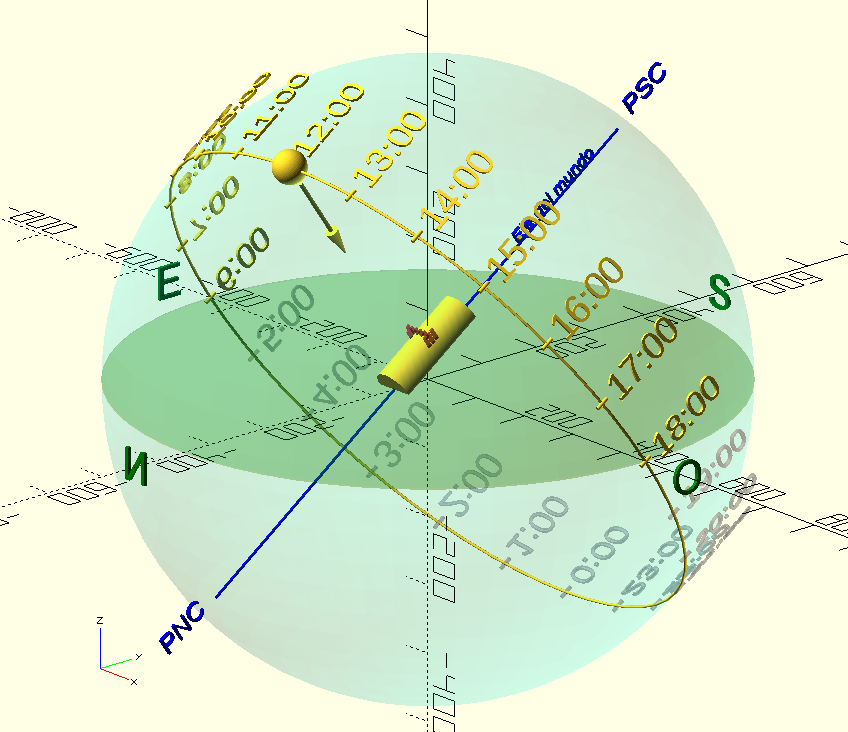
\includegraphics[width=.55\textwidth,valign=c]{imagenes/sol-culminacion-superior.png}\hfill
  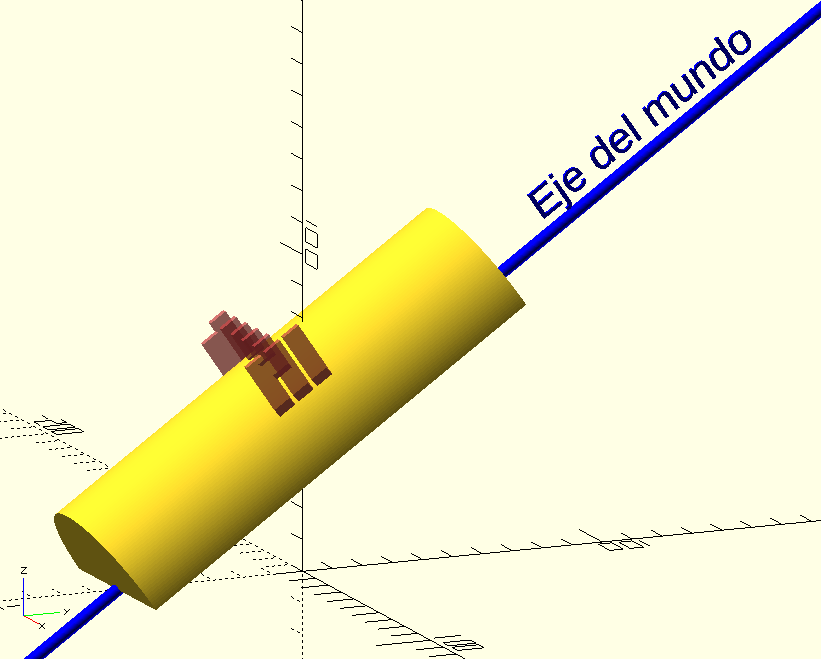
\includegraphics[width=.44\textwidth,valign=c]{imagenes/hora-12-alfa-90}
   \caption{A las 12 horas, el ángulo debe ser 90$^{\circ}$.}
  \label{fig:hora-12}
\end{figure}


---¡Sí! ---afirmó Cecilia, con entusiasmo---. A las 12 horas, el
ángulo debe ser de 90$^{\circ}$.

\begin{figure}[ht]
  \centering
  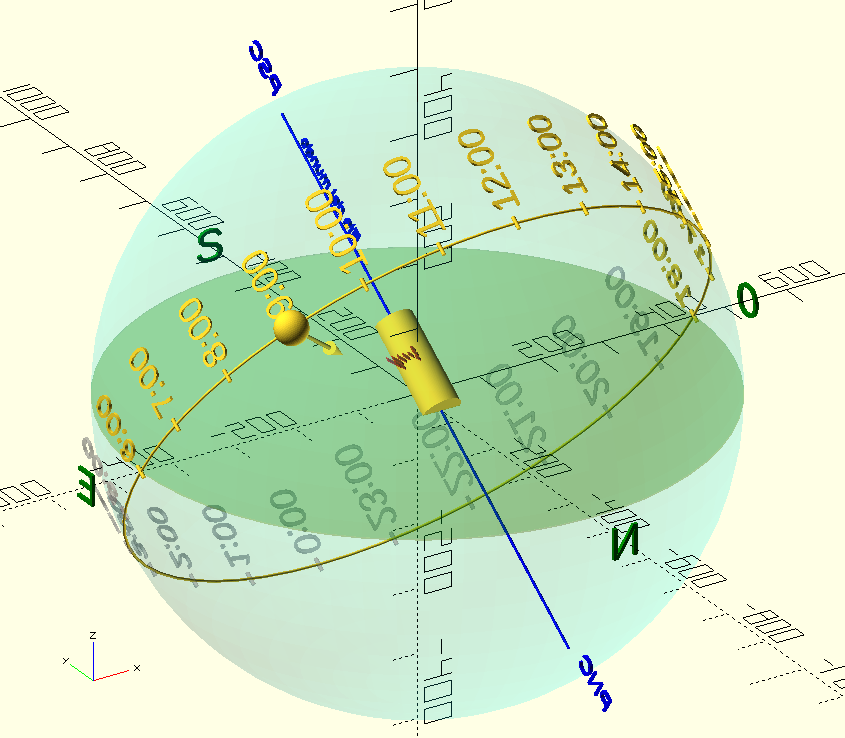
\includegraphics[width=.55\textwidth,valign=c]{imagenes/sol-9-horas.png}\hfill
   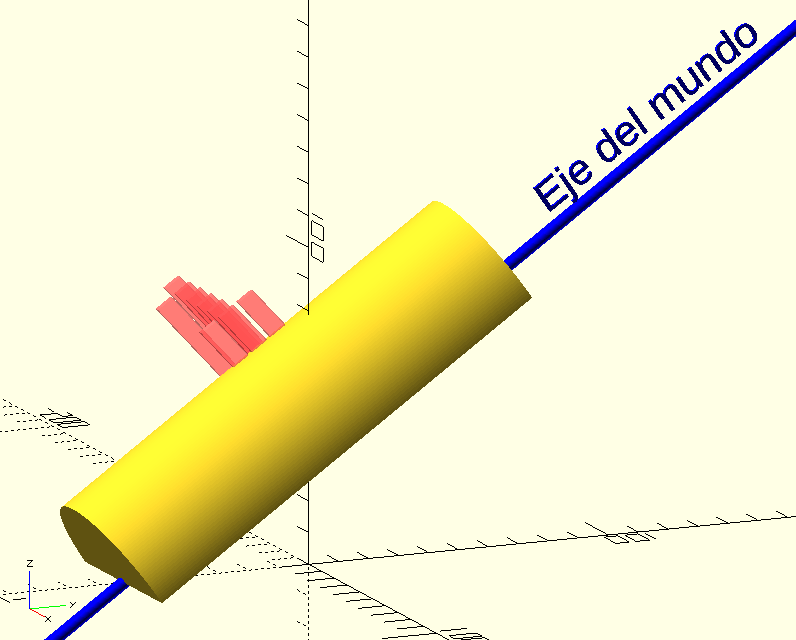
\includegraphics[width=.44\textwidth,valign=c]{imagenes/hora-9-alfa-135}  
   \caption{A las 9 horas, el ángulo debe ser 135$^{\circ}$.}
  \label{fig:hora-9}
\end{figure}

---Y a las 9 horas, 135$^{\circ}$ ---se apresuró Antonia a agregar con
una sonrisa.

\begin{figure}[h!]
  \centering
  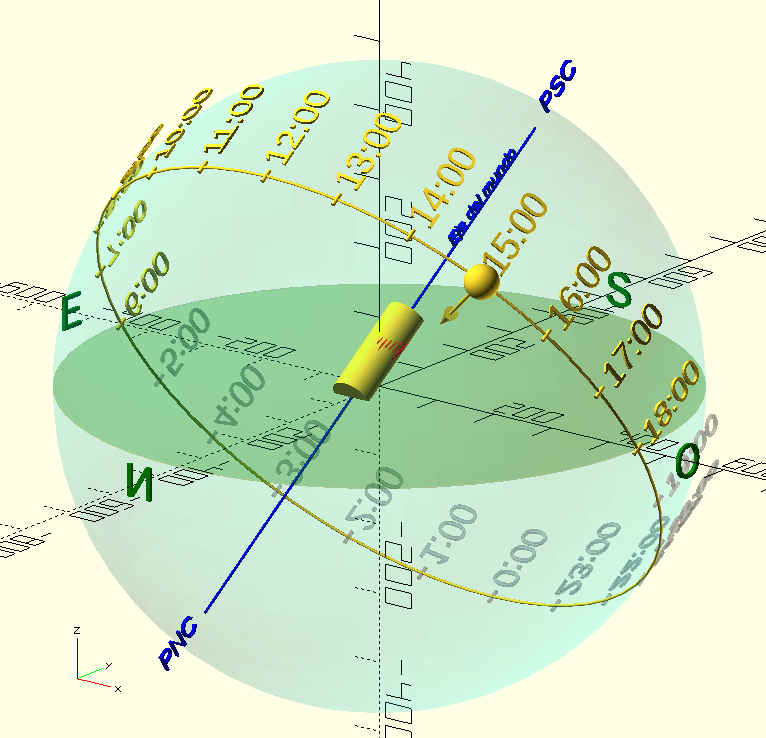
\includegraphics[width=.5\textwidth,valign=c]{imagenes/sol-15-horas.png}\hfill
   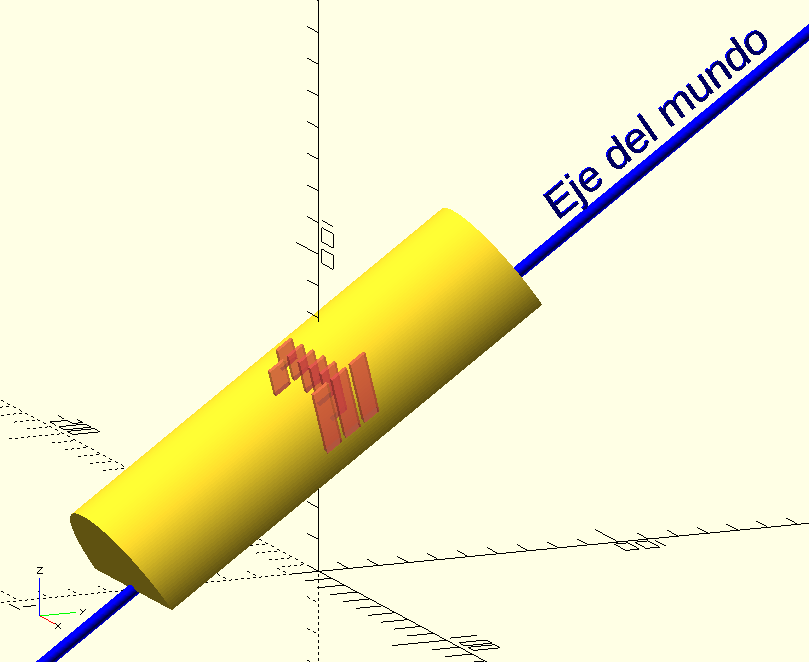
\includegraphics[width=.44\textwidth,valign=c]{imagenes/hora-15-alfa-45}  
   \caption{A las 15 horas, el ángulo debe ser 45$^{\circ}$.}
  \label{fig:hora-15}
\end{figure}

---¡Y a las 15 horas, 45$^{\circ}$! ¡Canté! ---gritó Cecilia, riendo.

---Perfectamente, entonces ---Antonia recapituló---; está claro que el
ángulo variará desde 180$^{\circ}$ hasta 0$^{\circ}$ conforme las
horas avanzan desde las 6:00 hasta las 18:00.
  
Cecilia sólo pudo expresar su acuerdo con una sonrisa: ¿estaría
emocionada por encontrarse más cerca de concretar el reloj?  ¿O sólo
cansada de pensar y caminar?  No lo sabía, y lo cierto es que poco le
importaba: en cualquier caso, la sensación que la embargaba ahora se
parecía mucho a la felicidad.

---Cuando volvamos a la oficina veremos cómo escribir matemáticamente
esa relación entre horas y ángulos que acabamos de establecer
conceptualmente ---anticipó Antonia, que también parecía querer
concluir el capítulo---. Pero me gustaría que discutiéramos un detalle
más. Fijate que establecimos esa relación para un sitio como Harvard,
cuya latitud es austral\footnote{¿Ignora acaso el autor que la célebre
  universidad de Harvard está ubicada en el hemisferio norte? (Nota
  del Editor)}$^,$\footnote{No entendiste nada.}: ¿Será la misma para
un sitio del hemisferio norte?

Cecilia se detuvo un instante antes de retomar el paso; efectivamente,
la cuestión era interesante en sí misma, pero además útil: sería muy
bonito que el reloj que estaban escribiendo pudiera concretarse en
cualquier sitio del planeta. Buscando nuevamente en su carpeta
encontró lo que buscaba: en la figura \ref{fig:mov-ap-sol-norte} podía
comprobarse que para el caso del hemisferio norte terrestre el este y
el oeste quedaban intercambiados en relación con el cuerpo del reloj;
por esa razón, para las latitudes boreales a las 9:00 le corresponde
un ángulo de 45$^{\circ}$, a las 15:00 uno de 135$^{\circ}$, etc.

\begin{figure}[t]
  \centering
  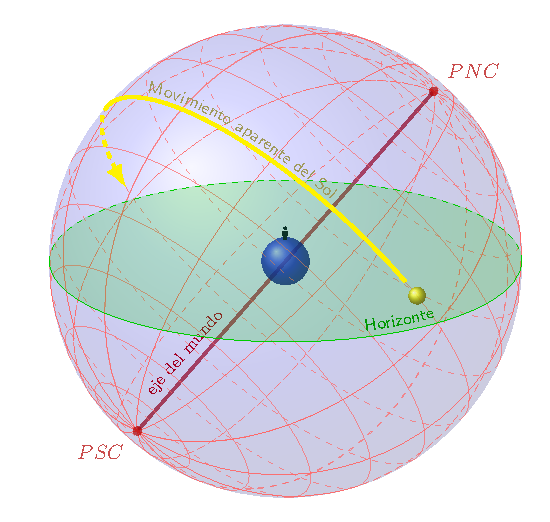
\includegraphics[width=.49\textwidth]{imagenes/movimiento-aparente-solar-hemisferio-norte}\hfill
  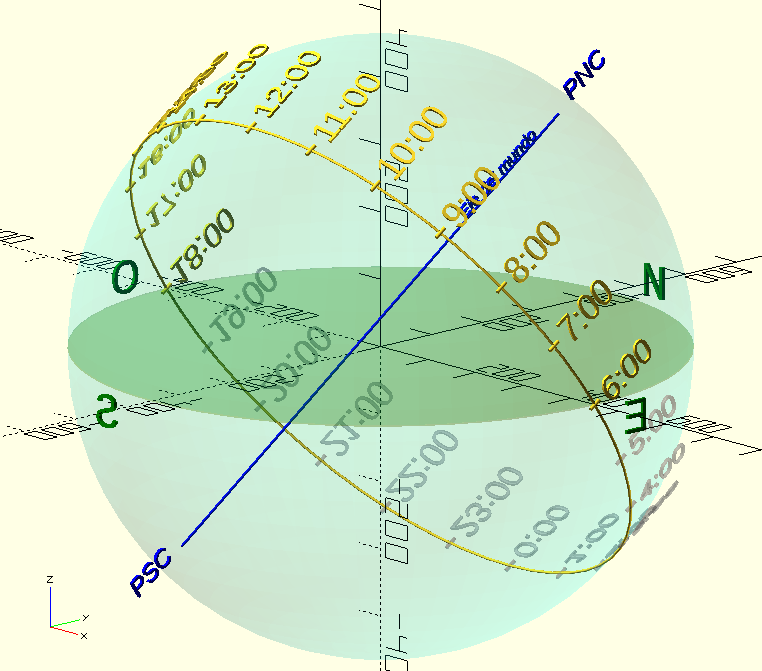
\includegraphics[width=.49\textwidth]{imagenes/esfera-celeste-horas-norte}
  \caption{Movimiento diurno aparente del Sol, tal como es apreciado
    por un observador ubicado en el hemisferio norte terrestre.}
  \label{fig:mov-ap-sol-norte}
\end{figure}


---No parece un problema muy difícil de resolver ---a\-ven\-tu\-ró
Cecilia---; supongo que deberemos escribir dos relaciones matemáticas
entre horas y ángulos: una para cada hemisferio. Y permitir que el
usuario indique, mediante una variable, si desea usar su reloj en el
norte o en el sur, y en función de eso emplear una u otra relación:
suena a una tarea para un \lstinline!if!.

Antonia sonreía mientras escuchaba y caminaba junto a Cecilia. Pensó
que ya empezaba a sonar como una programadora: elevando suposiciones
al rango de algoritmos, cifrando sentencias breves al borde de lo
confuso, y hasta enfrentando problemas aún no resueltos con una
confianza demasiado parecida a la pedantería. Por un momento temió
estar echándola a perder; pero decidió que, en cualquier caso, ya era
demasiado tarde.

Los últimos rayos de Sol conseguían aún filtrarse entre las hojas de
los añosos árboles de Harvard. La brisa era más fresca, y el color de
las hojas empezaba a desaparecer como desaparecen todos los colores al
caer la noche. Cecilia y Antonia, en su paseo, ya estaban llegando a
los pies de los muros de Harvard. Algunos astrónomos, cansados de su
trabajo diario, se asomaban por las altas ventanas y miraban con un
ligero desdén a las dos amigas que habían dedicado la tarde
aparentemente a pasear.

Antonia y Cecilia notaron esas miradas acusadoras; sin mediar palabra
entre ellas supieron inmediatamente qué debían hacer. Se separaron
unos pasos, y Antonia dio comienzo a la danza:

---Cecilia, ¿cómo era el movimiento aparente de las estrellas cuando
estamos ubicadas en un polo..?

Y ambas abrieron ceremoniosa y ampliamente los brazos, y ante los
escandalizados ojos de los astrónomos de Harvard comenzaron a girar, y
a girar, y a girar, mientras bailaban con las hojas y los árboles y la
brisa y los últimos rayos de Sol.






%%% Local Variables:
%%% mode: latex
%%% TeX-master: "../libro"
%%% End:
